\subsection{Organisering og økonomisk potensial}

\subsubsection{Organisering}

Den tenkte forretningsmodellen er å selge produktet til profesjonelle "radonjegere".
De betaler da en engangssum for én enhet.
Fordeler med dette kan være å ha høy inntjening tidlig, når man får solgt de første produktene.
Dette kan hjelpe på å skaffe kapital til å gjøre flere investeringer i utbedringer av produktet, og ekspansjon til flere markeder.
En ulempe kan være at det er vanskelig for mange kunder å gjøre en så stor engangsinvestering i et produkt, og at for mange ville muligens en modell med betaling over tid vært mer hensiktsmessig.
En slik måneds-/årspris kan være naturlig å kombinere med en supportavtale som inkluderer reparasjoner.
Her synes også et problem med modellen som baserer seg på en engangspris.
Dersom man får mange tilfeller av feil i produktet som må repareres, kan det bli dyrt å gjøre alle disse reparasjonene, med eventuelle tilbakekallinger av solgte enheter.
En løsning for å begrense omfanget av slike problemer, er å passe på at så mye som mulig av funksjonaliteten til enheter er implementert i programvare fremfor maskinvare.
Da er det lett å fikse uforutsette problemer ved å sende ut en programvareoppdatering.
Dersom enheten uansett har innebygd internett-tilkobling (for opplasting av data), er det trivielt å legge inn støtte for nedlasting av programvareoppdateringer i tillegg.

Teknologien til produktet stammer fra CERN, og de jobber sammen med personer fra Sintef med den videre utviklingen.
Det vil ikke være hensiktsmessig å bygge hele produktet selv fra grunnen av.
Selve mikrokontrolleren er det f.eks. mange firmaer som har spesialisert seg på å produsere, og det lønner seg derfor å kjøpe denne fra noen som leverer dette.
Det overordnede produkt-designet er noe man bør gjøre selv, men selve monteringen kan også med fordel outsources til noen som har erfaring og ekspertise på sammensetting av komponenter.

\textbf{Software:}
Uavhengig av om man går for en ren web-løsning, med direkte opplasting til internett fra enheten, eller om man velger en løsning hvor enheten sender data til en desktop-app, vil man trenge en programvareutvikler.
Men arbeidsmengden, og typen utvikling vil variere stort mellom disse to løsningene.
En desktop-løsning krever gjerne å lage applikasjoner for flere plattformer, slik som Windows, Mac og ev. Linux.
En ren web-løsning, derimot, kan være enklere å sette opp, og vil nok kreve mindre utviklingstid.

\subsubsection{Økonomisk potensial}

Årlig selges det 20 randonmålere i Norge. I en norsk sammenheng ønskes det å spise av dette markedet. Med et så snevert market blir det vanskelig i lengden å kunne ha en bærekraftig utvikling. Derfor er det ønskelig å starte i et større marked enn i Norge alene og rakst ekspandere til flere land. I USA er det 400 lisensierte randonmålere og dobbelt så mange ikke-lisensierte, ved å komme inn på et slikt marked kan man ha en bærekraftig ekspansasjon.

Skandinavia er et godt marked å starte i, alle de skandinaviske landene har nogelunde likt marked og det er ingen store kulturforskjeller som man må ta i betrakting. Man kan da senere brænde seg som en høyteknologisk bedrift fra skandinavia i andre markeder utad.

Produktet retter seg mot bedriftsmarkedet og er ikke et konsumerprodukt. Man vil derfor ha mulighet til å ha en god profittmargin. Det vil også være nødvendig for å overleve med et slikt produkt. Det vil ikke bli mange salg, i hvert fall ikke i startfasen.

Produktet beskrevet kan selges på markedet for rundt 30.000 NOK, dette er lik pris som konkurrentene. Av denne summen er det 20.000 NOK i ren profitt, så en profittmargin på $66,7 \%$.

Hvordan er denne profittmarginen satt med tanke på reell salgsforventning i første iterasjon av produktet?

\begin{table}[ht!]
    \begin{center}
    \begin{tabular}{ | l | r | }
        \hline
        Enheter produsert               & Totale kostnader per stykk \\
        \hline
        10                              & 10.000 NOK \\
        \hline
        Sum kostnad første iterasjon    & 100.000 NOK \\
        \hline
    \end{tabular}
    \end{center}
\end{table}

Nullpunktet til denne itrasjonen vil være på 100.000 NOK. Ved et forventet salgsvolum på 4 enheter á 30.000 NOK får man følgende regnestykke for risikomargin (Nåværende omsetning - Nullpunkt = Risikomargin).

$$ 120.000 - 100.000 = 20.000$$

og følgende for prosentmessig risikomargin:

$$ \frac{(120.000 - 100.000) * 100}{120.000} = 16,7 \% $$

Dette viser at ved 4 solgte enheter vil man ha 20.000 NOK i overskudd. Vidre får vi at med fire solgte enheter kan omsetningen synke $16,7 \%$ før man går i rent underskudd.

\begin{figure}[ht!]
    \begin{center}
    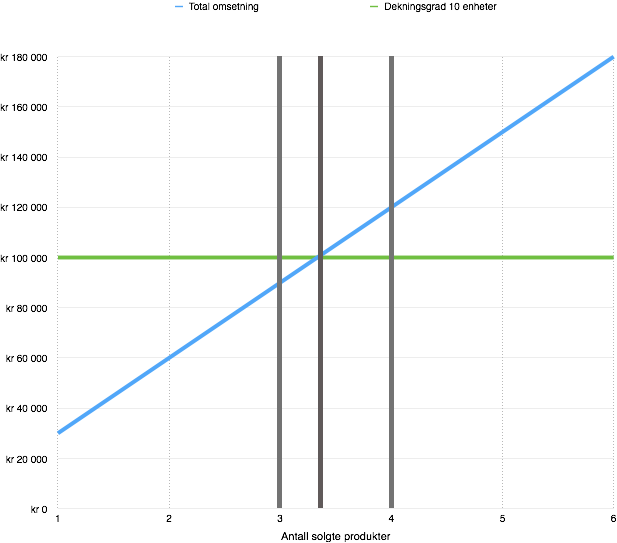
\includegraphics[width=0.5\textwidth]{graph.png}
    \label{fig:profitmargin}
    \end{center}
\end{figure}

Grafen på figur \ref{fig:profitmargin} viser hvordan man går i overskudd på 4 enheter og underskudd på 3 enheter. X-aksen er antall produkter solgt, Y-aksen er kroner i omsetning. Den grønne linja er kostnad for 10 produserte enheter. Den blå linja er total omsetning.

\textbf{Investeringsbehov:}
For å unngå høye investeringskostnader i starten har det blitt valgt å gjøre bindende avtaler med leverandører av komponenter til produktet. Disse avtalene går ut på å binde seg til disse leverandørene i lange tiderog dermed kunne få lave startkostnader. Dette vil lønne seg for begge parter hvis produktet går bra og viser at andre har tro på samme produkt.

\textbf{Investorer:}
Bedriften vi har snakket med er for tidlig i prosessen til å snakke med investorer, da det gjerne forventes at man kan vise til suksess i markedet før de er interesserte.
Veiledere de har snakket med om produktet er svært positive, og mener blant annet at det er en fordel at produktet inkluderer elementer av både teknologi og helse. Helse Midt-Norge er f.eks. en institusjon som deler ut midler til slike produkter, og kan være aktuell i fremtiden.
